\paragraph{Diagramme de classes de CANgateway}

\begin{minipage}
    {\linewidth}
    \centering
    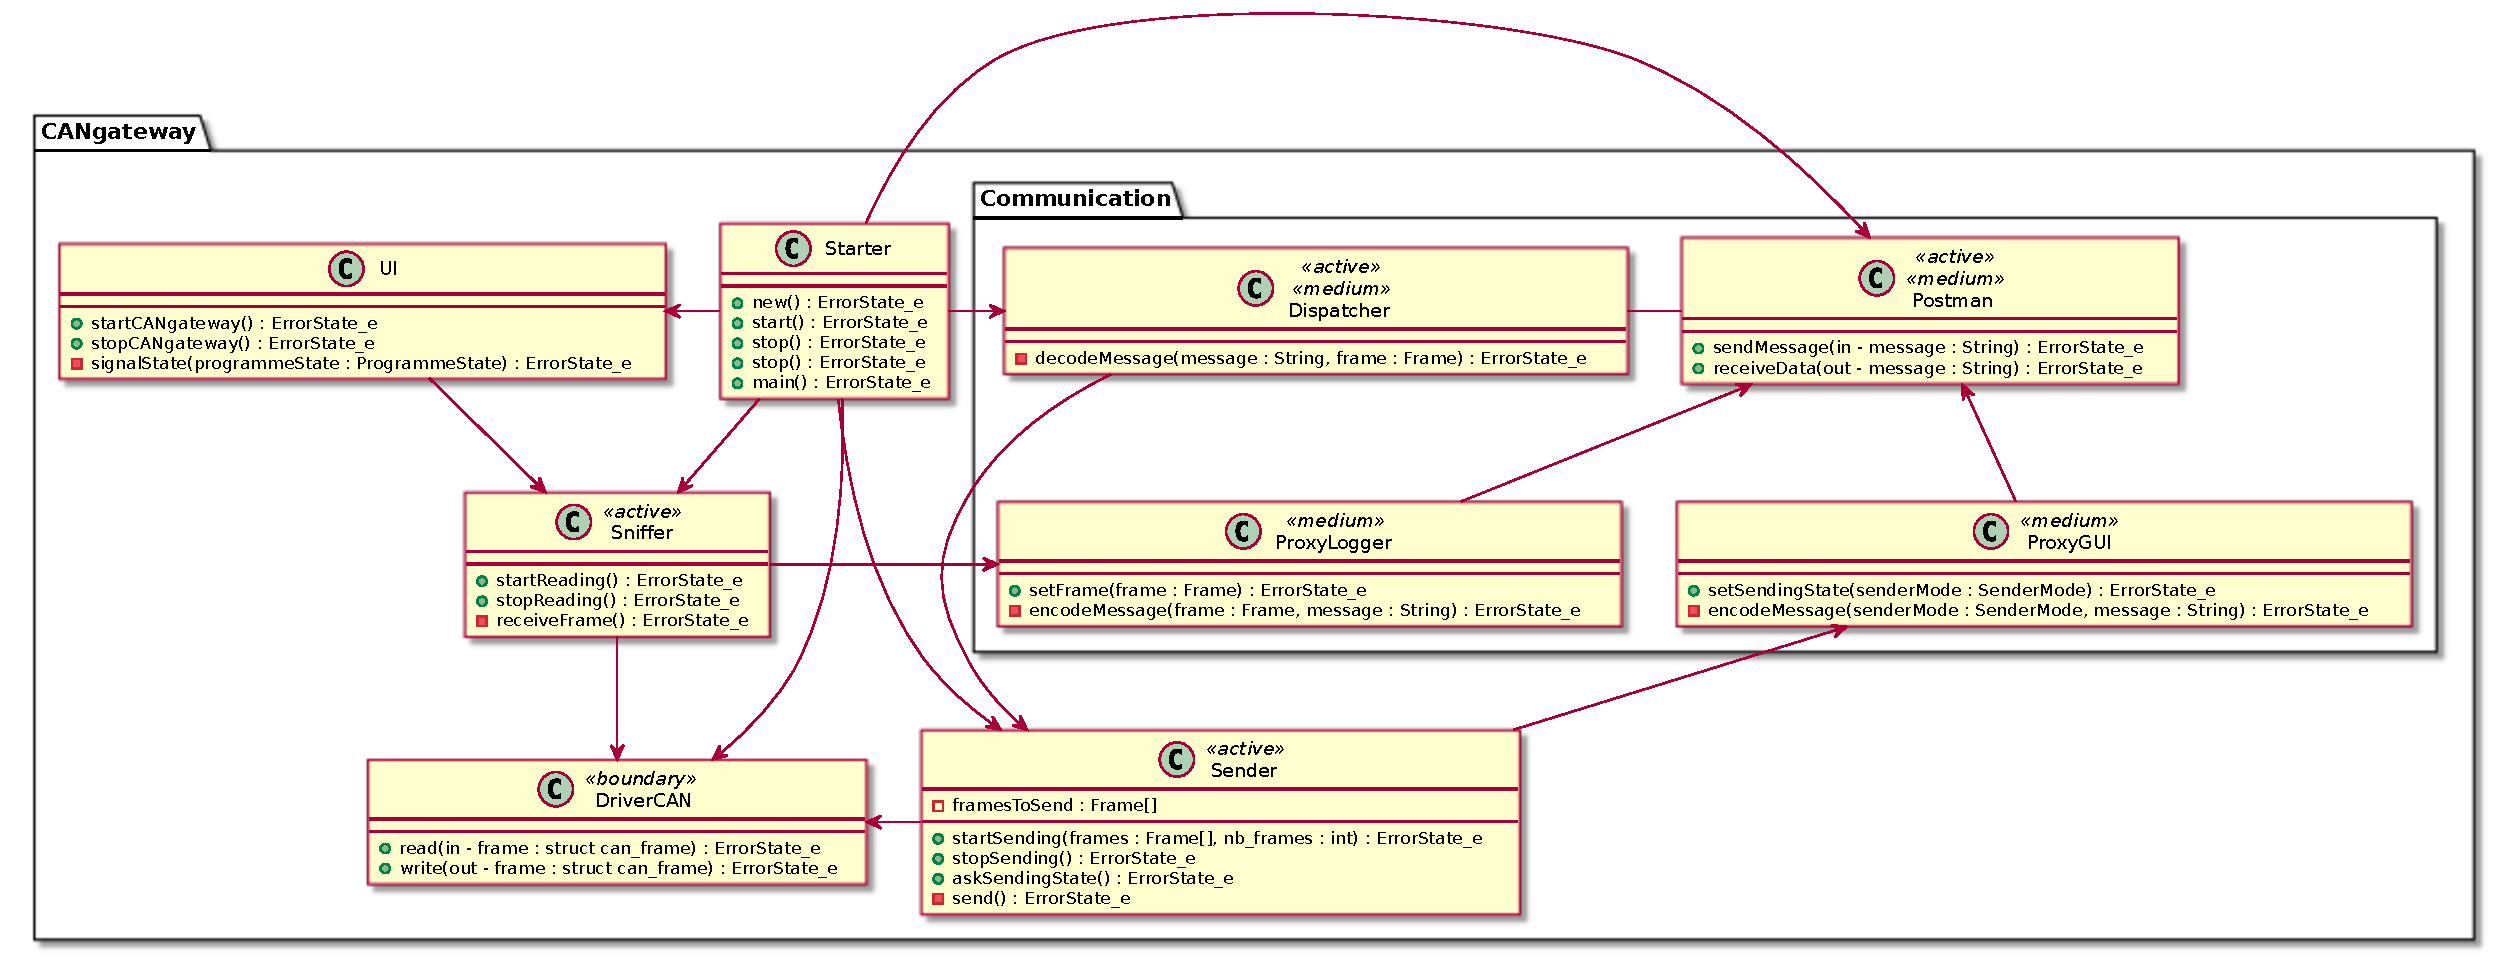
\includegraphics[width=\linewidth]{../schemas/Conception_detaillee/diag_classe_CANgateway.pdf}
    \captionof{figure}{Diagramme de classes de CANgateway}
\end{minipage}

\medspace

Le diagramme de classes de la figure ci-dessus représente l'architecture du programme {\nomLogiciel}. Cette architecture ne respecte pas totalement l'architecture de la conception générale due à l'implémentation d'une gestion d'erreur en C qui change donc les types de retours des fonctions. 
Ces fonctions retournent un état d'erreur de la forme : 
\begin{itemize}
    \item Enumération ErrorState\_e
    \item \'Eléments : 
    \item \begin{itemize}
        \item ERROR\_STATE\_SUCCESS : si tout se passe bien 
        \item ERROR\_STATE\_FAILURE : s'il y a au moins une erreur
        \item ERROR\_STATE\_TIMEOUT : si la cause de l'erreur est un timeout
    \end{itemize}
\end{itemize} 